\documentclass[a4paper,12pt]{article}
\usepackage[cp1250]{inputenc}
\usepackage[english]{babel}



\usepackage[pdftex]{graphicx}
\usepackage{amsmath}
\usepackage{listings}
\usepackage{xcolor}
\usepackage{color}


\setlength{\textwidth}{6.5in}
\setlength{\oddsidemargin}{0 cm}
\setlength{\evensidemargin}{0 cm}

\begin{document}

\begin{titlepage}
\begin{center}
\large Statistical Inference final assignment\\[1cm]
\LARGE A/B testing\\[1cm]
\large Author: Rok Bohinc \\
\large Basel, June 2019 \\[1 cm]
\end{center}

\begin{abstract}
In this work I analyze the  ToothGrowth data in the R datasets package and investigate the dependence of the ``len'' parameter on the ``dose'' and ``supp'' parameters. First, I perform an exploratory data analysis and plot the corresponding dependence, which helps me in formulating a hypothesis. Afterwards I perform hypothesis testing to confirm the observed differences in length of odontoblasts as a function delivery method of vitamin C.
\end{abstract}
\end{titlepage}


\section{Exploratory data analysis}

The "ToothGrowth" data set contains the data about  the length of odontoblasts (cells responsible for tooth growth) in 60 guinea pigs. Each animal received one of three dose levels of vitamin C (0.5, 1, and 2 mg/day) by one of two delivery methods, orange juice (coded as OJ) or ascorbic acid (a form of vitamin C and coded as VC). This information came together with description of the data set in R.

To investigate the tooth growth in guinea pigs I have performed a basic exploratory analysis. In Figure \ref{fig:Tooth1} I show box plots of tooth lengths as a function of vitamin C dose for the two delivery methods. Figure \ref{fig:Tooth2} additionally shows a scatter plot with linear regressions. From the two plots it is apparent that the tooth length increases  with the vitamin C dose (approximately linearly ) for both delivery methods. However, for orange juice delivery method the lengths seem to be higher for lower dose levels, i.e. 0.5 mg/day and 1 mg/day, than for ascorbic acid delivery method. 

\section{Hypothesis testing}

To verify this observation I have performed hypothesis testing. For H$_0$ hypothesis I take that there is no difference between the delivery methods for each dose level, whereas the alternative hypothesis H$_a$ I take that the corresponding differences are different from zero. As the number of observations is small I have employed the $t$ statistics, assumed an equal variance, and assumed that the observations are not paired. I choose a type I error rate of $\alpha=0.05$. The R code for performing the associate simulation is shown below.
\footnotesize
\begin{lstlisting}[backgroundcolor = \color{lightgray}, language=R]
data(ToothGrowth)

t.test(subset(ToothGrowth, dose == 0.5 & supp == "VC")$len, 
subset(ToothGrowth, dose == 0.5 & supp == "OJ")$len, 
paired = FALSE, var.equal = TRUE)

t.test(subset(ToothGrowth, dose == 1 & supp == "VC")$len, 
subset(ToothGrowth, dose == 1 & supp == "OJ")$len, 
paired = FALSE, var.equal = TRUE)

t.test(subset(ToothGrowth, dose == 2 & supp == "VC")$len, 
subset(ToothGrowth, dose == 2 & supp == "OJ")$len, 
paired = FALSE, var.equal = TRUE)

\end{lstlisting}
\normalsize
The code performs a $t$-test for the pairs of data sets for each dose level.

The $t$-tests for dose levels 0.5 mg/day, 1 mg/day, and 2 mg/day yield $p$-values of 0.005,  0.0008, and 0.96, respectively. As the first two values are smaller than $\alpha$ we reject H$_0$  for dose 0.5 mg/day and 1 mg/day, while for dose 2 mg/day we fail to reject H$_0$. This indicates that for the first two dose levels the lengths are different for different delivery methods.

\newpage
\section{Appendix}


\begin{figure}[!h]
\centering
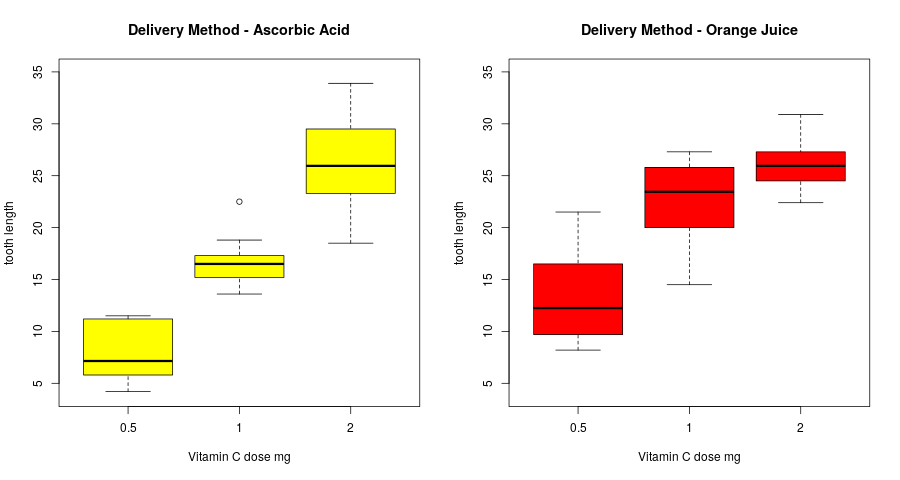
\includegraphics[width=13 cm]{Toothgrowth2.png}
\caption{ \label{fig:Tooth1}
Box plots of guinea pigs teeth as a function of dose levels of vitamin C  for orange juice (right plot) or ascorbic acid (left plot) delivery methods.}
\end{figure}

\begin{figure}[!h]
\centering
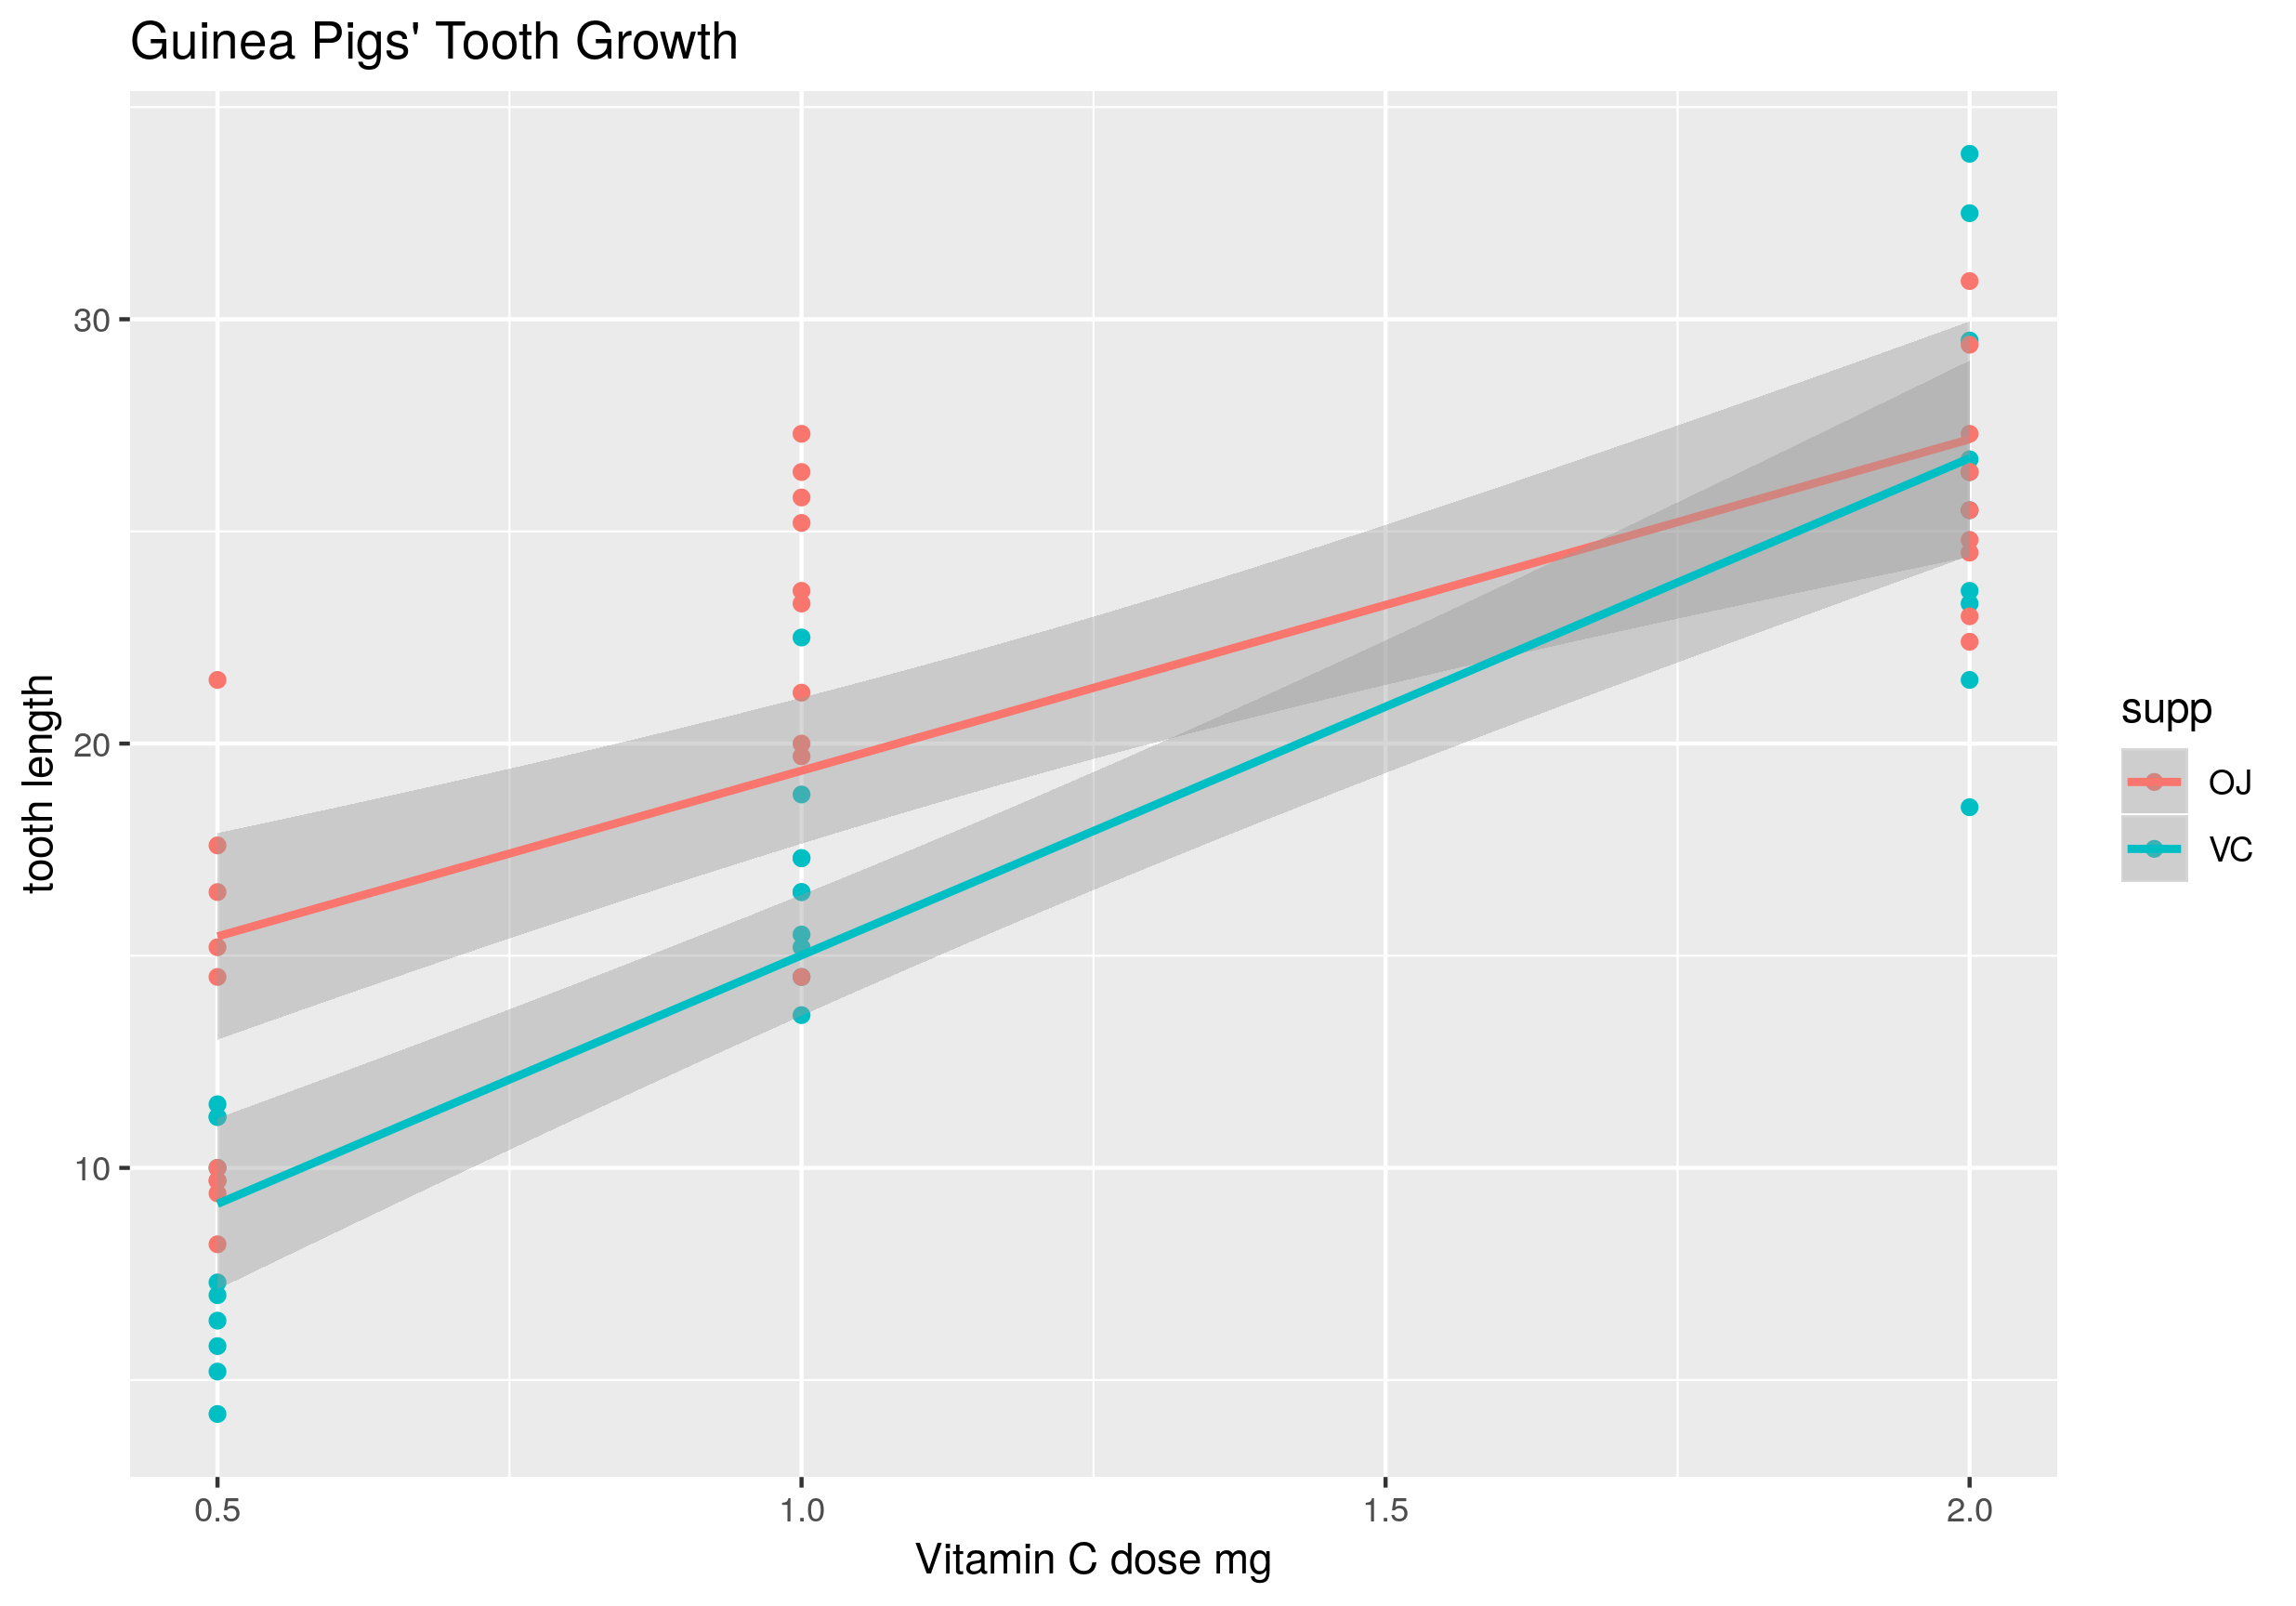
\includegraphics[width=11 cm]{Tootgrowth.png}
\caption{ \label{fig:Tooth2}
Length of odontoblasts as a function of dose levels of vitamin C  for orange juice (coded as OJ) or ascorbic acid (coded as VC) delivery methods. The solid lines represent the linear regression of the two data sets separated by the delivery method.}
\end{figure}


\end{document}


